% -*- TeX:SI -*-
% slovene sub-mode for spell check
% ----------------------------------------------------------------------
%  Predloga za obliko in navodila za pisanje diplomskih nalog v LaTex-u

%  Univerza v Ljubljani, Fakulteta za elektrotehniko

%  zbral in uredil Roman Kamnik, junij 2013

% ----------------------------------------------------------------------

\documentclass[a4paper,twoside,openright,12pt]{book}
\usepackage[latin2]{inputenc}  %Kodna stran za Windows okolje, za linux je kodna stran latin2
\usepackage[slovene]{babel}    % pravila za slovensko deljenje besed
\usepackage[pdftex]{UNI-LJ-FE-Diploma} %Stil za diplome na Fakulteti za elektrotehniko (za pdfTeX v MkiTex)
%\usepackage[pctex]{UNI-LJ-FE-Diploma} %Stil za diplome na Fakulteti za elektrotehniko  (za pcTex)


\usepackage{tikz}
\usetikzlibrary{calc}


\newcommand{\magnet}[3]{% xsredisce, ysredisce, zasuk
 \pgfmathsetmacro{\Cosa}{cos(#3)}
 \pgfmathsetmacro{\Sina}{sin(#3)}
\draw (#1,#2) circle (2);
\draw ( -2.0 * \Cosa  , -2.0 * \Sina )--(2.0 * \Cosa , 2.0 * \Sina );
\node at (-1.6*\Sina ,1.6*\Cosa ){\rotatebox{#3}{N}};
\node at (1.6*\Sina ,-1.6*\Cosa  ){\rotatebox{#3}{S}};
\fill (#1,#2) circle [radius=1pt] node [anchor=north east]{$S_m$};
}


\newcommand{\senzorja}[3]{% xsredisce, ysredisce, zasuk
 \pgfmathsetmacro{\Cosb}{cos(#3)}
 \pgfmathsetmacro{\Sinb}{sin(#3)}



\hall{#1+2.4*\Cosb }{#2+2.4*\Sinb }{#3}
\hall{#1-2.4*\Sinb}{#2+2.4*\Cosb}{#3}
\fill (#1,#2) circle [radius=1pt] node [anchor=south east]{$S_h$};

\draw [dashed, thick](#1,#2)--(#1+2.2*\Cosb ,#2+2.2*\Sinb );
\draw [dashed, thick](#1,#2)--(#1-2.2*\Sinb ,#2+2.2*\Cosb );
}

\newcommand{\hall}[3]{

 \pgfmathsetmacro{\Cosd}{cos(#3)}
 \pgfmathsetmacro{\Sind}{sin(#3)}
 
\draw 
(#1 - 0.2 * \Sind -0.2 * \Cosd  ,#2 + 0.2 * \Cosd -0.2 *\Sind )--
(#1 - 0.2 * \Sind +0.2 * \Cosd  ,#2 + 0.2 * \Cosd +0.2 *\Sind )--
(#1 + 0.2 * \Sind +0.2 * \Cosd  ,#2 - 0.2 * \Cosd +0.2 *\Sind )--
(#1 + 0.2 * \Sind -0.2 * \Cosd  ,#2 - 0.2 * \Cosd -0.2 *\Sind )--
(#1 - 0.2 * \Sind -0.2 * \Cosd  ,#2 + 0.2 * \Cosd -0.2 *\Sind );

\draw (#1-0.1,#2+0.1) --(#1+0.1,#2-0.1);
\draw (#1+0.1,#2+0.1)-- (#1-0.1,#2-0.1);
}


%*************************** PRILAGODITVE *****************************
% mapa s slikami
\potgrafike{./Slike/}
%prilagoditev levega roba sodih strani. �e se pri dvostranskem tisku robovi ne umemajo se lahko pove�a ali pomanj�a
\zamaknirobsodihstrani{0mm}

%*************************** NASLOVNA STRAN *****************************
\naslov{Vpliv stat�ne in dinami�ne ekscentri�nosti na napako senzorja RM44, u�inkovitost kalibracije in robustnost kalibracije na harmonske oscilacije mehanske hitrosti}
\avtor{Mitja Ali�} \univerza{Univerza v Ljubljani}
\fakulteta{Fakulteta za elektrotehniko}
\delo{Magistrsko delo}
%\delo{Diplomsko delo visoko�olskega strokovnega �tudija}
\date{Ljubljana, 2017}
\mentor{doc. dr. Mitja Nemec}
%\somentor{prof. dr. Ime Priimek}
\begin{document}

%------------------------ ZA�ETNI DEL -----------------------------------
%\frontmatter
%%------------------------------------------------------------------------
%
%
%%************************ NASLOVNA STRAN ********************************
%\maketitle
%
%
%%*************************** ZAHVALA ************************************
%\zahvala V zahvali se kandidati zahvali mentorju in poimensko tudi
%vsem sodelavcem in prijateljem, ki so pomagali in prispevali pri
%delu v laboratoriju, na ra�unalniku, v delavnici, pri tehni�ni
%izdelavi dela in drugje.
%
%
%%*************************** VSEBINA *************************************
%\tableofcontents
%
%%*************************** SEZNAM SLIK in TABEL  ***********************
%\seznamslik
%\seznamtabel
%
%%***************************  SEZNAM UPORABLJENIH SIMBOLOV  **************
%
%\seznamsimbolov
%
%V pri�ujo�em zaklju�nem delu so uporabljeni naslednje veli�ine in
%simboli:
%
%\begin{table}[h]
%\centering
%%\begin{footnotesize}
%\begin{tabular}{l l l l}
% \hline \multicolumn{2}{c}{\bf{Veli�ina / oznaka}} & \multicolumn{2}{c}{\bf{Enota}}  \\
% \hline
%Ime & Simbol & Ime & Simbol \\
% \hline
% �as & $t$  & sekunda & s \\
% frekvenca & $f$  & Hertz & Hz \\
% tlak & $p$  & Pascal & Pa \\
% sila vzgona & $\textbf{\textit{f}}_\text{vz}$  & Newton & N \\
% gostota & $\rho$  & - & kg/m$^3$ \\
% masa telesa  & $m_\text{t}$  & kilogram & kg \\
% vhodna napestost & $U_\text{vh}$ & volt  & V \\
% Jacobijeva matrika & $\mathbf{J}$  & - & - \\
%  \hline
%\end{tabular}
%%\end{footnotesize}
%  \caption{Veli�ine in simboli}
%  \label{prebojne_trdnosti}
%\end{table}
%
%
%
%%------------------------ GLAVNI DEL ------------------------------------
%\mainmatter
%%-------------------------------------------------------------------------
%
%
%%********************* POVZETEK V SLOVEN��INI ****************************
%\povzetek
%
%V pri�ujo�em delu so predstavljena navodila za izdelavo 
%
%\kljucnebesede beseda1, beseda2, beseda3
%
%
%%*************************** POVZETEK V ANGLE��INI ***********************
%\abstract
%
%The thesis addresses ...
%
%\keywords word1, word2, word3
%
%
%%***************************** UVOD **************************************
%\chapter{Uvod} \label{uvod}
%
%Uvod v zaklju�no delo ima namen, da uvede bralca v tematiko
%zaklju�nega dela. V njem kandidat raz�leni zahteve in cilje
%zaklju�nega dela, po literaturi povzame znane 
%re"sitve in oceni
%njihov pomen za zaklju�no delo. Sklicevanje na literaturo se v
%besedilu ozna�i s "stevilko v oglatem oklepaju, ki jo ima ta v
%seznamu uporabljenih virov, in po potrebi navede strani, npr.
%\cite{miklavvcivc2010objavljanje} ali \cite[stran 520 -
%534]{juvznivc1992diplomska}.
%
%%*********************** OSREDNJA POGLAVJA ********************************
%\chapter{Izbira teme zaklju�nega dela} \label{izbira_teme}
%
%\chapter{Princip delovanja senzorja RM44}
%
%
%
%
%\chapter{Dolo"canje napake s simulacijo}




\chapter{Vpliv ekscentri"cnosti}

Idealna postavitev magneta in senzorja na os vrtenja je v realnosti te"zko dose"ci. Od tod lo"cimo dva tipa ekscentri"cnosti, ki si ju bomo pogledali v nadaljevanju. Njihov vpliv ni vedno zanemarljivo majhen. Napake zaradi ekscentri"cnosti se pojavijo zaradi nenatan"cne vgradnje v postroje. 


V za"cetnem delu kjer sem sestavil model z Matlab-~om, sem 




, v tej nalogi pa se bom osredoto"cil na izredno majhne premike. 


\begin{figure}
\centering
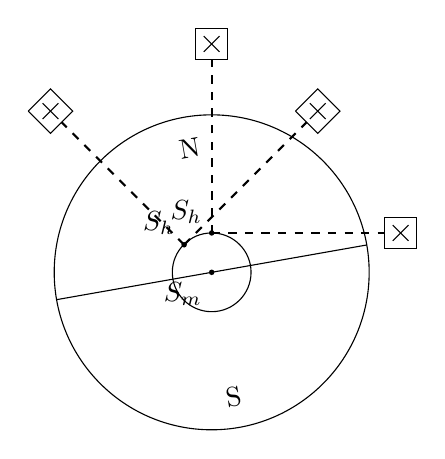
\begin{tikzpicture}[scale=1]
\magnet {0} {0} {10}
\senzorja{0}{0.5}{0}
\draw (0,0) circle (0.5);
\senzorja{-0.35}{0.35}{45}

\end{tikzpicture}
\caption{Prikaz navora v odvistnosti od komponent toka }

\label{fig:navor}
\end{figure}
%izpeljava ekscentricnosti za 1 senzor [x0,y0]

\section{izpeljava stati"cne ekscentri"cnosti}
%Napises da je senzor izmaknjen iz centra magneta in sredisce senzorja opise kroznico
%
%
%
%
%\section{izpeljava dinami"cne ekscentri"cnosti}
%napisi da je magnet izmaknjen senzor pa zavrtis okoli sredisca senzorja






%\section{Rezultati simulacij}
%
%\chapter{Zaklju�ek} \label{zakljucek}
%
%
%


\end{document}
